%% LaTeX2e class for student theses
%% sections/content.tex
%% 
%% Karlsruhe Institute of Technology
%% Institute for Program Structures and Data Organization
%% Chair for Software Design and Quality (SDQ)
%%
%% Dr.-Ing. Erik Burger
%% burger@kit.edu
%%
%% Version 1.3.2, 2017-08-01


\chapter{Adaptive Monitoring for Continuous Performance Model Integration}
\label{ch:Adaptive Monitoring for Continuous Performance Model Integration}
In this chapter, we will introduce our approach for adaptive monitoring for continuous performance model integration. In section \ref{sec:Context of our approach}, we bring in the context of our approach. In section \ref{sec:Monitoring Probes}, we define the monitoring probes that we need for our monitoring approach. In section \ref{sec:Monitoring Records}, we define the monitoring records that we monitor. In section \ref{sec:Adaptive Instrumentation}, we clarify the adaptive instrumentation concept in our approach. In section \ref{sec:Instrumentation Model}, we define an instrumentation for saving the monitoring probes. In section \ref{sec:approach}, we give an overview approach an it's activities. In section \ref{sec:Monitoring Probes Generation Process}, we introduce the process that we used to generate iteratively the monitoring probes. In section \ref{sec:Adaptive Instrumentation Process}, we present our approach for adaptive instrumentation of the source code. 

\section{Context of our approach}
\label{sec:Context of our approach}
As mentioned before, our approach is part of the CIPM vision (Section \ref{sec:Continuous Integration of Performance Model}) which extends the agile and DevOps process and provides them with iterative and incremental Performance Model. Moreover, the Performance Models in CIPM are enriched with Performance Model Parameters. In the following, we will briefly depict and describe the process and the context in which our approach takes place.\\

Figure \ref{fig:Context of our approach} shows the process in which our approach takes place. this process is based on Vitruvius (Section \ref{sec:Vitruvius}) which means its elements are either models or transformations. The Java code in \ref{fig:Context of our approach} is represented by a JaMoPP model. When the developer commits changes on this model, two transformations will be triggered. The first one is the Coevolution process of Langhammer (Section \ref{sec:Automated Coevolution of Source Code and Software Architecture Models}) which keeps the Source Code and the models in the Palladio Component Model consistent, mainly the repository and the SEFF Model. The second Transformation is our Transformation which is specified for keeping the Source Code and the Instrumentation Model consistent. We proposed the Instrumentation Model in order to persist the Probes that will be required for instrumenting the Source Code.\\

When the system under development is deployed, our Instrumentation Process will be triggered. This process receives as inputs the Probes from the Instrumentation Model and the Source Code of the System. It delivers afterwards the instrumented Source Code as a JaMoPP Model. After the instrumentation process has been finished, the instrumented Source code will be executed and monitored.  The information provided by monitoring are encapsulated in a Measurement Model which describes the needed monitoring records.  After the monitoring has been finished the Parameters Estimation Process (Section sec:Iterative Performance Model Parameter Estimation Considering Parametric Dependencies) can be triggered. it uses the information in the Measurement Model to estimate the Performance Model Parameters and updates accordingly the SEFF Model in the Palladio Component Model. Afterwards, the user can use the updated Performance Model to simulate and evaluate the performance of the system. \\


\begin{figure}[h]
\centering
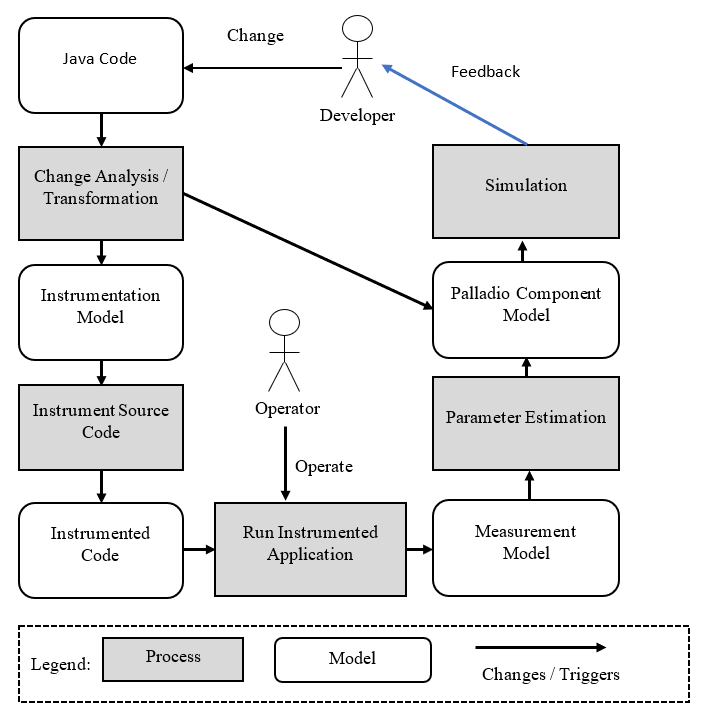
\includegraphics[width=0.9\textwidth]{figures/approach_context}
\caption{Context of our approach}
\label{fig:Context of our approach}
\end{figure}


\section{Monitoring Probes}
\label{sec:Monitoring Probes}
Monitoring Probes are responsible for collecting monitoring information from the system. Furthermore, they can be specified based on the needed monitoring information. For example, if we need to monitor the response time of a service and the number of execution of loops, we can specify two monitoring probes, one probe for the response time and the other for loops execution number. \\

In our approach, we want to provide monitoring information for Palladio Performance Model which are described in terms of SEFF (Section \ref{sec: SEFFs}).   SEFF Model is composed from four main elements which inherit from the so-called Abstract Action, namely Internal Action, Branch Action, Loop Action and Service Call Action. In other words, we should specify probes that provide these elements with the needed monitoring information. Therefore, we defined a monitoring probe for each SEFF element Figure \ref{fig:Specified Monitoring Probes in our Approach}. The monitoring information that we need to produce for SEFF elements are described in (Section \ref{sec:Monitoring Records}) under monitoring records.  \\

For the monitoring purpose, we used the Kieker Monitoring Framework (Section \ref{sec:Kieker Monitoring}) which offers the possibility to define new monitoring probes based on the needed monitoring records.\\

\begin{figure}[h]
\centering
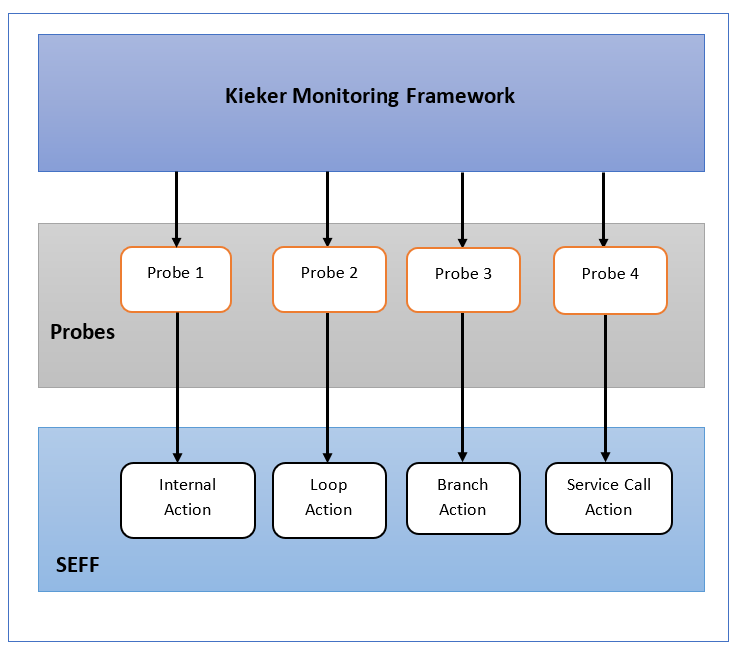
\includegraphics[width=0.9\textwidth]{figures/probes}
\caption{Specified Monitoring Probes in our Approach}
\label{fig:Specified Monitoring Probes in our Approach}
\end{figure}

\section{Monitoring Records}
\label{sec:Monitoring Records}
In order to create monitoring probes (Section \ref{sec:Monitoring Probes}), one must define first of all the needed monitoring information. in our case, we defined monitoring probes for SEFF model which are based on the monitoring records in Figure \ref{fig:records}. \\

Figure \ref{fig:records} shows an UML Class Diagram that describe the monitoring records. It provides extra information that are needed for the purpose of performance model parameters estimations. The abstract class RecordWithSession specifies a sessionID attribute that helps to identify the monitoring information based on sessions.  The abstract class ServiceContextRecord adds a serviceExecutionID attribute that helps to reference a ServiceCallRecord.\\

All records are identified via their ids. The id of each record can be provided by the used monitoring framework. However, in order to be able to use these records for SEFF models we've used for each record the id of the corresponding SEFF element. \\

For internal actions which express internal computation, we want to know the time consumed by them. Therefore, we need to log the id of the internal action, start time and stop time. \\

For Loops, we need to recognize the number of executions of a loop. The same thing for branches, we log the id of the executed branch in order to realise if the branch was executed or not. \\

As to service calls, we need to locate them in which service are called, we need also to provide the response time and the parameters they are given. The parameters of services are given in a JSON format.\\

\begin{figure}[h]
\centering
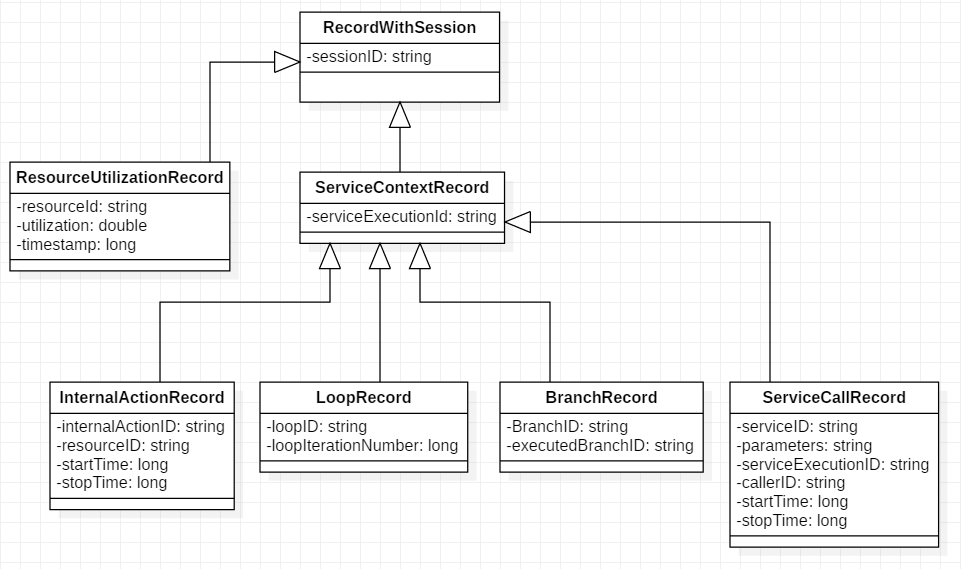
\includegraphics[width=0.9\textwidth]{figures/records}
\caption{UML class diagram that shows the monitoring information required by SEFF models}
\label{fig:records}
\end{figure}

\section{Adaptive Instrumentation}
\label{sec:Adaptive Instrumentation}
In this section, we will introduce the meaning of Adaptive Monitoring in our approach as well as the main concepts used in order to achieve that.\\

As mentioned before, our approach is addressed to iterative development processes like DevOps. In this context, Adaptive Instrumentation means that only the parts of the source code that have been changed in the current iteration will be monitored. \\

Based on this definition, we should be able to generate instrumentation points during the development phase. In order to do this, we decided to use two main concepts which are model-driven engineering and change-driven engineering. Moreover, our approach is based on the Coevolution approach which itself uses these two concepts to keep the source code and the architecture models consistent. Precisely, the Coevolution approach uses change-driven consistency preservation in order to keep the Java source code and SEFF models consistent. Changes in the source code model are monitored and transformed to changes in the SEFF model based on defined consistency-preservation rules. \\

In order to achieve an adaptive instrumentation in our approach, we’ve defined and Instrumentation Model which contains the instrumentation points. Moreover, we defined a transformation that monitored changes in the source code model and creates the corresponding instrumentation points in the instrumentation model. \\

In order to keep the source code and the instrumentation model consistent, we've used Vitruvius Framework which makes it possible to keep models instances consistent based on models changes. 

\section{Adaptive Monitoring}
\label{sec:Adaptive Monitoring}
Adaptive Monitoring means that the monitoring probes can be activated and deactivated based on the existing monitoring information. this is needed when we’ve collected enough monitoring information for some probes but they still can log monitoring information which is not needed and which can lead to monitoring and performance model parameters estimations overhead.  Therefore, adaptive monitoring can help to reduce the monitoring overhead by reducing the number of monitoring probes. \\

In order to achieve Adaptive Monitoring in our approach, we've added an attribute for the monitoring probes that defines their activeness. That means, monitoring probes are checked during the monitoring phase and they can log monitoring information only if the are activated. The deactivation of the probes can be done for example, when we've realised that the current monitoring information for these probes are enough for the performance model parameters estimation.\\

\section{Instrumentation Model}
\label{sec:Instrumentation Model}
The Instrumentation Model was originally presented in the approach of Manar and Koziolek \cite{mazkatli2018continuous} on which we based our approach. 

The Instrumentation Model (IM) Figure \ref{fig:im} is one of the Contribution of this thesis in Vitruvius. IM is responsible for describing and managing the instrumentation points. Moreover, we've defined IM in order to achieve the Adaptive Instrumentation (Section \ref{sec:Adaptive Instrumentation}) and Adaptive Monitoring (Section \ref{sec:Adaptive Monitoring}).\\

IM is composed from two elements, AppProbes which represents the model root and the element Probe which represents an instrumentation point. The element Probe corresponds to a SEFF abstract action which can be an Internal Action, a Branch Action, a Loop Action or a Service Call Action.\\

As mentioned before, we’ve used Vitruvius in order to keep the source code and the IM consistent. We've also extended the Coevolution approach which uses also Vitruvius to keep the Java source code and the architecture models consistent. The Coevolution approach uses an instance of the SEFF model in which our probes are stored. Therefore, in order to avoid redundant information within Vitruvius, we've decided to store only the Ids of these probes which give us the possibility to return them when they are needed. Moreover, since the probes represent concretely the four above mentioned abstract actions of SEFF, the id of a probes is named abstractActionID. Furthermore, we've added a boolean attribute to the monitoring probes in order to enable to adaptive monitoring. \\

\begin{figure}[h]
\centering
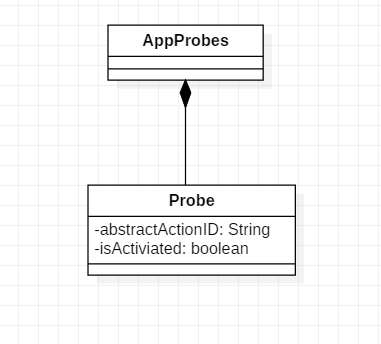
\includegraphics[width=0.5\textwidth]{figures/im}
\caption{UML Class Diagram that represents the Instrumentation Model}
\label{fig:im}
\end{figure}


\section{Approach}
\label{sec:approach}
In this section we will briefly introduce our approach as well as the context in which our activities will be executed. Further details on these activities will be presented in the next chapters.\\

our approach is developed in the context of the iterative development process DevOps. Therefore, Figure \ref{fig:devops_approach} gives an overview of the activities of our approach and in which DevOps phase they can be executed. The green color indicates processes or model in which our algorithms are executed. \\

In our approach we've defined to main processes. The first one is responsible for collecting the instrumentation points or the probes. It must be executed during the development phase. It uses information from Vitruvius and it's based on the Coevolution approach. The Coevolution approach keeps the source code and the SEFF model consistent and provides us with information that help to gather the probes. Vitruvius is used to keep the source code model and the Instrumentation Model consistent. The generated probes are saved and managed in the Instrumentation Model. For more details on the probes generation process, look at the chapter (Probes Generation Process).\\

The second process is the instrumentation process which can be executed at any time. Once it's executed, it takes the probes from the Instrumentation Model and insert the instrumentation source code in the source code of the system based on the types of the probes (Figure 2). However, if the monitoring will be firstly done in the monitoring phase of DevOps, this process can be automatically triggered at the Continuous Deployment phase. For more details on our instrumentation process look at the chapter (Source Code Instrumentation Process).\\

In the monitoring phase, the instrumented system can be executed in order to log monitoring information. Moreover, in order to achieve an adaptive monitoring, the monitoring probes execute a self-checking for their activeness. Therefore, the monitoring code uses information from the Instrumentation Model in order to check if probes are activated of deactivated and thus if they can log or not. \\


\begin{figure}[h]
\centering
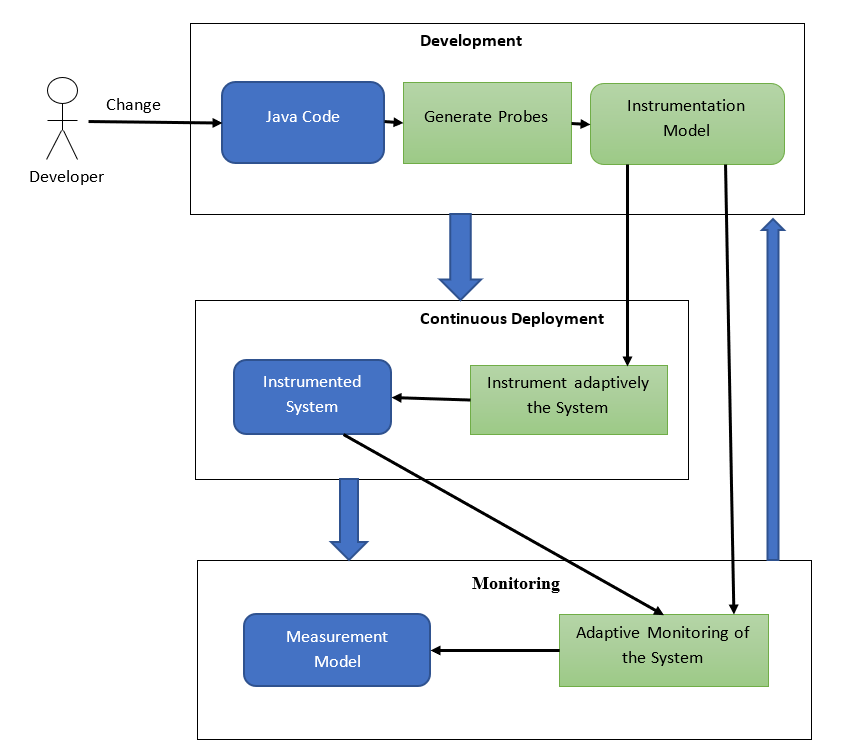
\includegraphics[width=0.9\textwidth]{figures/devops_approach}
\caption{Overview of our Approach Activities in DevOps context}
\label{fig:devops_approach}
\end{figure}

\section{Monitoring Probes Generation Process}
\label{sec:Monitoring Probes Generation Process}
As mentioned before, we used the Vitruvius Framework and change-driven approach to create the probes in order to achieve the adaptive instrumentation. Moreover, we showed that the generation of the monitoring probes is equivalent to keeping the source code model and the instrumentation model consistent. the consistency between these models is realised within Vitruvius.\\

In this section, we will introduce our approach for the monitoring probes generation as well as the collection of the information that is needed for the instrumentation process. In section \ref{sec:Terminology}, we introduce the concepts that are used in our approach. In section \ref{sec:The Vitruvius VSUM of our approach}, we present the Vitruvius VSUM of our approach. In section \ref{sec:Collecting Information for the Transformation}, we describe how we collect the information that we need in our approach and the transformation that keeps the source code and the instrumentation model consistent. In section \ref{sec:Limitation}, we provided an overview of the limitation of our approach.\\

\section{Terminology}
\label{sec:Terminology}
In this section, we present the terminologies and the concepts we use to achieve the goals of our approach. In section \ref{sec:Source Code Decorator Model}, we present the Source Code Decorator Model. In section \ref{sec:Correspondence Meta-model}, we introduce the Correspondence Meta-model of the Vitruvius Framework. In section \ref{sec:Vitruvius VSUM}, we clarify the Virtual Single Underlying Model of Vitruvius. 

\subsection{Source Code Decorator Model}
\label{sec:Source Code Decorator Model}

The Source Code Decorator Model (SCDM) has been presented within the SoMoX approach (section \ref{sec:Source Code Model eXtractor}).  SoMoX reverse-engineers the source code and can extracts the architecture models from it. Moreover, SoMoX can be used to extract the Palladio Component Model (PCM) from the Java Source Code. The SCDM is used to create trace links at the model level. The linking between the source code elements and the architecture model elements are needed in the reverse-engineering process. Therefore, the SCDM creates links between the source code elements and the PCM elements. Furthermore, due to the use of SCDM, the reverse-engineering process can be done without mixing the linking concerns with the domain specific language of the source code model and the architecture model.\\

The SCDM was also used in the Coevolution approach (Section \ref{sec:Automated Coevolution of Source Code and Software Architecture Models}) which keeps automatically the Java Source Code and the PCM models consistent during the system development. The SCDM was used to contain the information, which source code element is reverse-engineered into which architectural model element. For example, it contains the information, which classes are mapped into which component.\\

In our approach we will need the SCDM in order to map between the SEFF elements and the source code elements or the statements. As mentioned before, the instrumentation points in our approach are represented by the SEFF elements. Moreover, in order to insert the instrumentation code in the right location in the source code of the system, we need to know which SEFF elements corresponds to which source code statements. The SCDM offers this possibility by mapping between each SEFF element and the corresponding JaMoPP statements. \\

In order to map between the SEFF elements and the JaMoPP statements, we do not need to implement this feature because it's done already in the Incremental SEFF Reconstruction Process (section \ref{sec:Incremental SEFF Reconstruction}) in the Coevolution approach. This process can monitor the changes within the source code and reconstructs incrementally the SEFF models. Moreover, the execution of this process requires the execution of the SoMoX in order to reverse-engineer the changed parts of the source code. The execution of SoMoX creates the SCDM which maps between the SEFF elements (like Branch Actions, Internal Actions, etc.) and the JaMoPP statements Figure \ref{fig:seff jamopp}.


\begin{figure}[h]
\centering
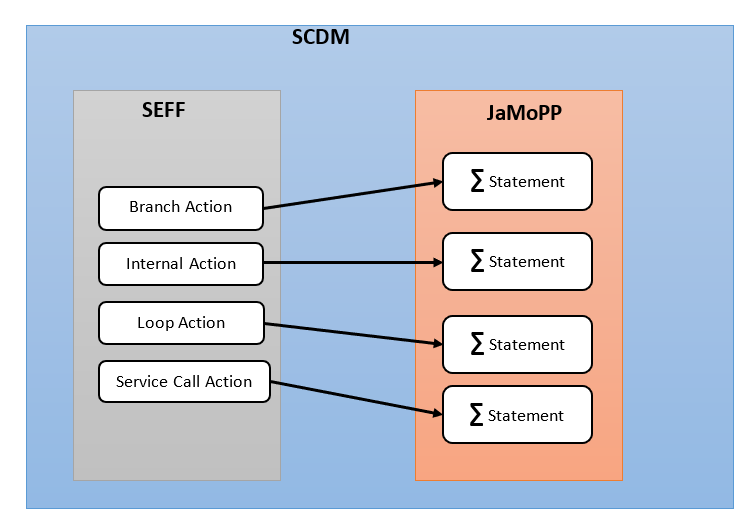
\includegraphics[width=0.9\textwidth]{figures/seff_jamopp}
\caption{Source Code Decorator Model (SCDM) maps between the SEFF Elements and the corresponding JaMoPP statements}
\label{fig:seff jamopp}
\end{figure}



\subsection{Correspondence Meta-model}
\label{sec:Correspondence Meta-model}
The Correspondence Metamodel (CMM) is used within Vitruvius in order to describe the corresponding elements of two meta-models. Moreover, Vitruvius one instance of CMM can be used for each Vitruvius application. A Vitruvius application can have one or many meta-models instances.  In our approach, we use one CMM instance which has been created and used in the Coevolution approach. Furthermore, for the process of probes generation we will use the existing information in this instance that have been saved the Coevolution approach and add new information to it by extending the Coevolution approach.\\

Figure \ref{fig:correspondence_model} shows the Vitruvius Correspondence Meta-model. It's basically composed from two classes. The root class Correspondences contains the list of Correspondence. The class Correspondence is composed from two list of identifier references. The first list contains identifiers that reference models in one meta-model, while the second list contains identifiers that reference models in the other meta-model.\\

CMM is a generic and can be used for diverse meta-models. Therefore, in order to identify an element, the reference in the Correspondence has to be unique because only one concrete element needs to be identified for a given ID. For this purpose, the CMM uses the so-called Temporarily Unique Identifier (TUID) mechanism. TUID is a string that can identifies an element. It has to be calculated based on the properties of the element that it represents. The TUID is also used when an element needs to be retrieved from the correspondence model.    

\begin{figure}[h]
\centering
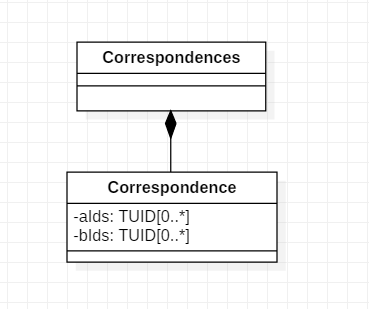
\includegraphics[width=0.9\textwidth]{figures/correspondence_model}
\caption{The Correspondence Meta-model of the Vitruvius Framework}
\label{fig:correspondence_model}
\end{figure}



\subsection{Vitruvius VSUM}
\label{sec:Vitruvius VSUM}
In order to keep models instances consistent, Vitruvius approach uses the so-called Virtual Single Underlying Model (VSUM) which contains all information that represents the system Figure \ref{fig:vitruv_vsum}. The models in VSUM are accessible using views. Views are instances of view types and they can be used to manipulate model instances. Moreover, there are two kinds of view types, namely projectional view types or combining view types \cite{burger2013flexible}. Projectional view types allows to show information from one meta-model solely. Combining view types can be used to show information from diverse meta-models.\\

Models consistency in Vitruvius can be preserved using Consistency preservation rules. They describe how changes in one model should be transferred into changes in another model. Moreover, the Consistency Preservation Process uses these rules to create the models transformation that preserves the consistency.\\


\begin{figure}[h]
\centering
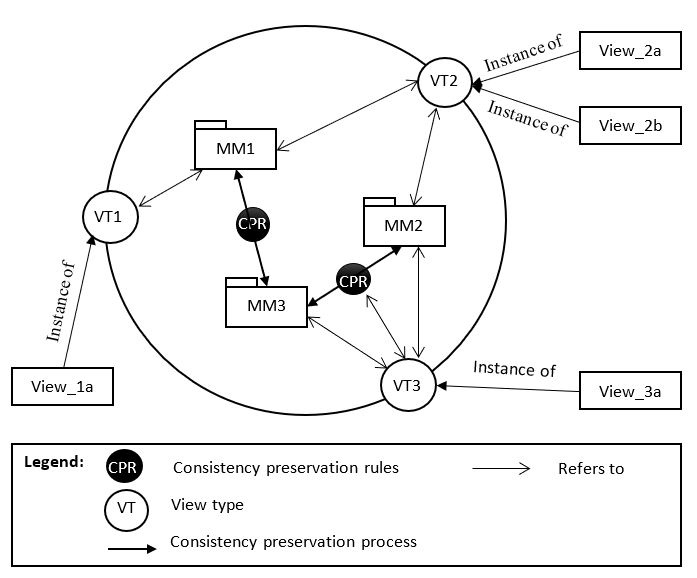
\includegraphics[width=0.9\textwidth]{figures/vitruv_vsum}
\caption{Overview of the Vitruvius VSUM and how model instances can be kept consistent}
\label{fig:vitruv_vsum}
\end{figure}



\section{The Vitruvius VSUM of our approach}
\label{sec:The Vitruvius VSUM of our approach}

In this section, we will present the VSUM of our approach in order to generate the monitoring probes. We will precisely extend the VSUM Figure (Section \ref{fig:coevoloution approach}) defined by the Coevolution approach.\\

As mentioned above, our approach extends the Coevolution approach, which keeps the source code and the architecture consistent. The VSUM in the Coevolution approach is composed from the following models:
\begin{itemize}
\item Palladio Component Model: it represents the architecture models.
\item JaMoPP Model: it represents the source code of the system.
\item Correspondence Model: it links between diverse model elements.
\end{itemize}
Moreover, the steps that are used to keep these models consistent are described in (Section \ref{sec:Automated Coevolution of Source Code and Software Architecture Models}). \\

In order to use Vitruvius for the adaptive monitoring purpose, we added an Instrumentation Meta-model (Section \ref{sec:Instrumentation Model}) that saves the monitoring probes and keeps them consistent with the source code. Figure \ref{fig:extended_vsum} shows our VSUM which is extended from the VSUM of the Coevolution approach. The steps described in (Section \ref{sec:Automated Coevolution of Source Code and Software Architecture Models}) are kept the same. However, we added a transformation (Section \ref{sec:Keeping the Source Code and the Instrumentation Consistent}) in the step (5) which keeps the Java source code and the instrumentation model consistent. 

\begin{figure}[h]
\centering
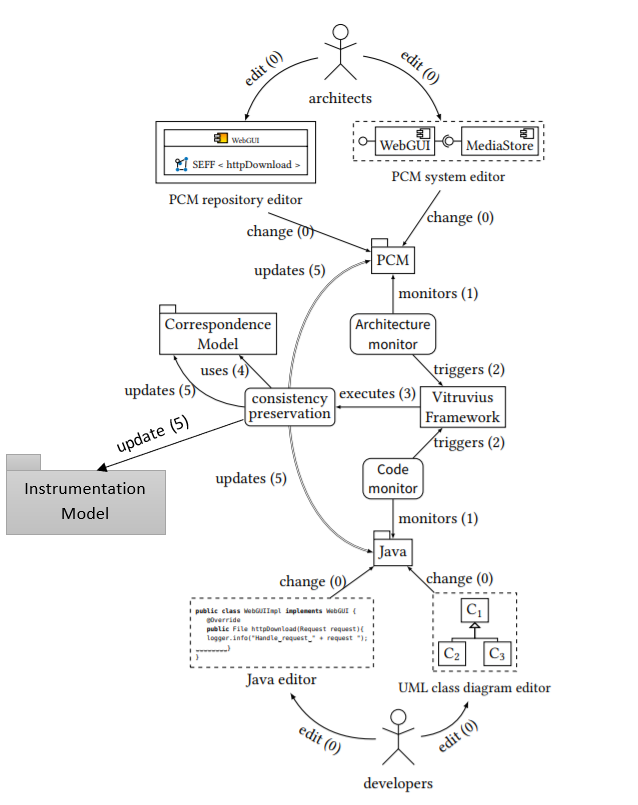
\includegraphics[width=0.9\textwidth]{figures/extended_vsum}
\caption{Overview of the Vitruvius VSUM of our approach, we extended the VSUM of the Coevolution approach}
\label{fig:extended_vsum}
\end{figure}

\section{Monitoring probes generation}
\label{sec:Monitoring probes generation}
In this section, we will introduce the process that we used to create the monitoring probes based on the Vitruvius Framework. This process is divided into two steps. The first step consists of collection the information that is useful for our transformation that keeps the source code and the Instrumentation Model consistent. the second step is the execution of this transformation.

\subsection{Collecting Information for the Transformation}
\label{sec:Collecting Information for the Transformation}
In this section, we present the process used to collect information. this information is can be used in the Instrumentation Process and for executing the transformation that generates the monitoring probes and keeps the source code and the instrumentation model consistent.\\

In order to execute our transformation, we need to know the new or the updated probes (SEFF elements).  For the Instrumentation Process we need the correspondence between the SEFF elements and corresponding JaMoPP statements. This information should be provided in each change of the source code. \\

In order to get this information, we used the information provided by the Incremental Reconstruction Process of SEFF (Section \ref{sec:Incremental SEFF Reconstruction}). This process reconstructs incrementally the SEFF of a service if its source code has been changed. Moreover, the SEFF elements are linked with the corresponding services in the Correspondence Model and can be retrieved from our transformation.\\

The second information that we need is the correspondence between the SEFF elements and source code. this information can be also provided by the SEFF reconstruction process. As described in (Section \ref{sec:Incremental SEFF Reconstruction}), the SoMoX is executed to reverse-engineer the changes service and creates its SEFF. SoMoX creates also the Source Code Decorator Model (SCDM) (Section \ref{sec:Source Code Decorator Model}) which contains links the SEFF elements of the service and the corresponding JaMoPP statements. Moreover, in order to make this information useful in our instrumentation process, we should make it accessible from outside of the SEFF reconstruction application. Therefore, we extended the SEFF reconstruction process with a new step that transforms the linking between the SEFF elements and the JaMoPP statements from SCDM into correspondences in the correspondence model Figure \ref{fig:seff_reconst_extension}. \\


\begin{figure}[h]
\centering
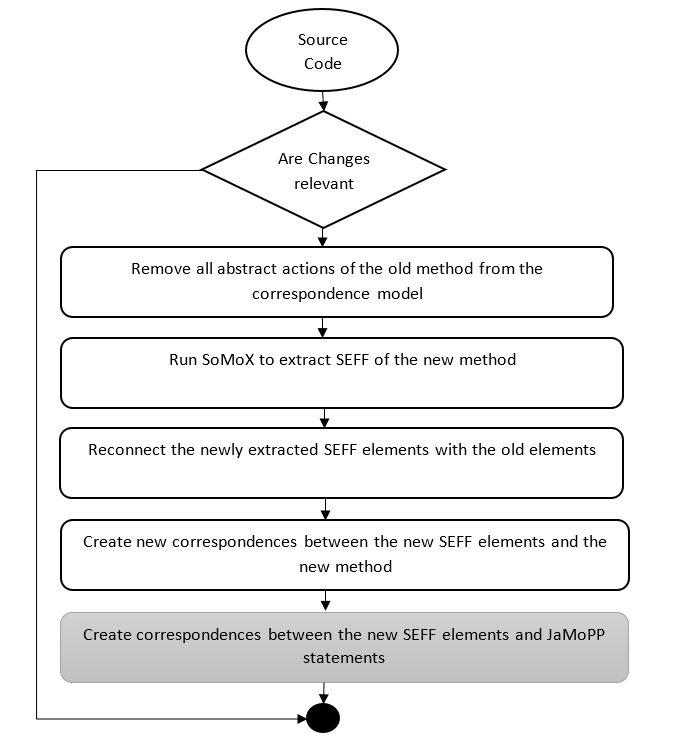
\includegraphics[width=0.9\textwidth]{figures/seff_reconst_extension}
\caption{The extended Incremental Reconstruction Process of SEFF}
\label{fig:seff_reconst_extension}
\end{figure}


\subsection{Keeping the Source Code and the Instrumentation Consistent}
\label{sec:Keeping the Source Code and the Instrumentation Consistent}
In this section, we present our transformation that keeps the source code and the Instrumentation Model (Section \ref{sec:Instrumentation Model}) consistent.\\

In order to generate the monitoring probes in our approach, we should preserve the consistency of the source code and the instrumentation model. Therefore, we created a transformation that transfers changes in the source code into changes in the instrumentation model. This transformation is executed when the source code has been changed.\\

In order to execute our transformation, we need to know the old service and its SEFF elements as well as the new service and its SEFF elements. This information can be obtained from the Correspondence Model after the Coevolution has been executed. Therefore, the Coevolution approach and our transformation are executed asynchronously. That means, we execute firstly the Coevolution approach in order to collect the information for our transformation then we execute our transformation based on this information.\\

The consistency preservation rules in our transformation are simple. When the source code has been changed and the changes are relevant, we delete the old probes of the old service from the instrumentation model and we add the new probes of the new service in the instrumentation model. Moreover, the new added probes are by default activated (Section \ref{sec:Monitoring Probes}). \\

\section{Adaptive Instrumentation Process}
\label{sec:Adaptive Instrumentation Process}
As we described in (Section \ref{sec:approach}), our approach is composed from two main activities. the first activity is responsible for collecting the monitoring probes. The second activity is the instrumentation process, which uses the collected monitoring probes from the first activity to instrument the source code. In this section, we define our Instrumentation Process for adaptive instrumentation of the source code.
 
\subsection{Design}
\label{sec:Design}
In this section, we give an overview from outside of our adaptive instrumentation process. In section \ref{sec:Inputs}, we define the inputs for this process. In section \ref{sec:output}, we discuss the alternative Outputs of our process and prove our decision. 
\subsection{Inputs}
\label{sec:Inputs}
Figure \ref{fig:approach_design} shows an overview of the inputs and the output of our Instrumentation Process. It receives three Inputs. First of all, the source code of the system which we want to monitor. secondly, The Correspondence Model which contains correspondences between the services and their SEFFs as well as correspondences between the SEFF elements and the corresponding JaMoPP statements. Finally, the Instrumentation Model which contains the instrumentation points that we should use to instrument the source code. 

\begin{figure}[h]
\centering
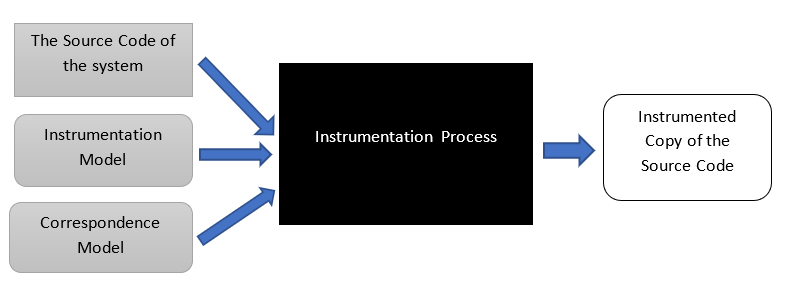
\includegraphics[width=0.9\textwidth]{figures/approach_design}
\caption{The inputs and the output of the instrumentation process, the output is an instrumented copy of the original source code of the system}
\label{fig:approach_design}
\end{figure}

\subsection{Output}
\label{sec:output}

The output of the Instrumentation process is an instrumented version of the source code of the system.  This instrumentation is based on the monitoring probes defined in (section Probes in the chapter approach). Moreover, there are two ways to instrument the source code. The first alternative consists of using the Aspect Oriented Programming which separate the instrumentation code from the source code of the system. The second alternative consists of mixing the instrumentation code with the source code of the system. Furthermore, we showed in (Section \ref{sec:Kieker Monitoring}) that the first alternative can not be used in our approach because of the fine-grained monitoring probes that we defined in our approach (section monitoring probes in the chapter approach). Therefore, we decided to use the second alternative in our instrumentation approach.\\

\textbf{Alternative of the instrumentation process outputs}\\
As mentioned above, in order to do the source code instrumentation, we decided to mix between the source code and the instrumentation logic.  Here, we distinguish also between two alternatives for instrumenting the source code of the system. The first alternative consists of instrumenting the original source code of the system. The second alternative consists of making a copy of the original source code of the system and instrument it. We decided to use the second alternative in our instrumentation process. \\

\textbf{Instrumentation of a copy of the source code}\\
The reason why we decided to use the second alternative to instrument the source code was due to the readability of the original source code. Moreover, if we instrumented the original source code of the system, we will reduce its readability and make the maintenance more difficult in the feature for programmers. Figure \ref{lst:instrumented_code} shows an instrumented version of the source code in Figure \ref{fig:Example of source code and SEFF}. As we can see, the readability of the source code has become difficult and the maintenance will be also hard to do. Therefore, we decided the instrument a copy the original system in order to receive the monitoring information.


\begin{lstlisting}[caption={Instrumented version of the source code in Figure \ref{fig:Example of source code and SEFF}, the instrumentation is the result of the execution of our approach},label={lst:instrumented_code}, captionpos=b, language=java] 
  class ComponentA{
        private componentB; 
        
        void service(boolean condition,
                       List array){        
            ServiceParametersFactory serviceParametersFactory = new ServiceParametersFactoryImp();
		    ServiceParameters __serviceParameters7b0c60ab_1116_477e_b9aa_6409dc557bb5 = serviceParametersFactory
				.getServiceParameters(new Object[] { condition, array }, new String[] { "condition", "array" });
		    ThreadMonitoringController.getInstance().enterService("_sPEbUDkyEembGJ6iNCoQDQ",
				__serviceParameters7b0c60ab_1116_477e_b9aa_6409dc557bb5);
                
            // internal computation
            final long __tin_f7087098_bbc8_4043_b1a3_e489deb8c13a = ThreadMonitoringController.getInstance().getTime();
            innerMethod_1();
            ThreadMonitoringController.getInstance().logResponseTime("_tWldADkyEembGJ6iNCoQDQ", "_oro4gG3fEdy4YaaT-RYrLQ",
				__tin_f7087098_bbc8_4043_b1a3_e489deb8c13a);
            
            // Branch Action
            String __executedBranch_91862b17_279e_4025_99c5_1610bb6dc5da = null;            
            if(condition){
                __executedBranch_91862b17_279e_4025_99c5_1610bb6dc5da = "_tXW5EDkyEembGJ6iNCoQDQ";
                ThreadMonitoringController.getInstance().setCurrentCallerId("_tXeN0DkyEembGJ6iNCoQDQ");
                componentB.service_1();
            }
            else{
                __executedBranch_91862b17_279e_4025_99c5_1610bb6dc5da = "_tXW5EDkyEembGJ6iNCoQDQ";
                long __counter_346b00f9_23d0_4e68_a582_15925d8a030a = 0;
                for(item in array){
                    __counter_346b00f9_23d0_4e68_a582_15925d8a030a++;
                    ThreadMonitoringController.getInstance().setCurrentCallerId("_nXeN0DkyHdnbGJ6iNCoQDW");
                    componentB.service_2();
                }
                ThreadMonitoringController.getInstance().logLoopIterationCount("_tXbKgDkyEembGJ6iNCoQDQ",
					__counter_346b00f9_23d0_4e68_a582_15925d8a030a);
            }
            ThreadMonitoringController.getInstance().logBranchExecution("_tXVD4DkyEembGJ6iNCoQDQ",
				__executedBranch_91862b17_279e_4025_99c5_1610bb6dc5da);
            ThreadMonitoringController.getInstance().exitService();   
        }
        
        private innerMethod_1(){
            // internal computation
            // ...
        }
        
    } 
\end{lstlisting}


\subsection{Architecture}
\label{sec:architecture}
Figure \ref{fig:architecture} describes the architecture of our Instrumentation approach. The component diagram shows the dependencies between the components that we used to implement our approach. \\

\textbf{Two Main Concerns}\\
We distinguish between two main concerns, which are executed in diverse contexts. The first concern is related to the instrumentation of the source code. The second concern consists of the logic used to extract the services parameters and to log the monitoring information.  \\

\textbf{The Source Code Instrumentation Concern}\\
In order to instrument the source code, we provided an instrumentation process which is implemented in the component \textit{Source Code Instrumentation}. This component depends on the component \textit{Probes Provider}, which provides the fine-grained probes (Section \ref{sec:Monitoring Probes}) we defined for our instrumentation approach. The component \textit{Source Code Instrumentation} uses these probes in combination with information from the Correspondence Model(Section \ref{sec:Correspondence Meta-model})to accomplish the instrumentation of the source code. we provide more details on the instrumentation process can be found in (Section \ref{sec:Call Sequence of the Instrumentation Process}.\\


\textbf{The Monitoring Source Code Concern}\\
This concern is related to the source code that has to be executed to log the monitoring information. it can be divided into two tasks. The first one consists of the extraction of the service parameters. This task is implemented by the components \textit{Service Parameters Extractor} and \textit{Service Parameters Factory}. The first component is responsible for extracting the service parameters values and their names and pass them to the second component. The second component receives the services parameters and put them in a defined format, currently it produces a JSON file, which contains the service parameters names as the keys that their values as the values of the keys. The second task consists of the logic used to collect and log the monitoring information, which is implemented in the component \textit{Monitoring}. The component \textit{Source Code of the System} represents the source code that we want to instrument, it has dependencies to the components \textit{Monitoring} and \textit{Service Parameters Factory}.\\ 

\begin{figure}[h]
\centering
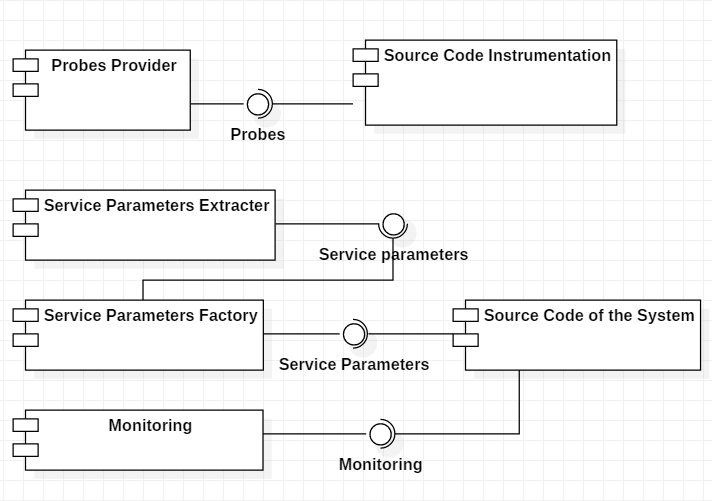
\includegraphics[width=0.9\textwidth]{figures/architecture}
\caption{The Component Diagrams shows the dependencies between the components we used to implement our approach}
\label{fig:architecture}
\end{figure}

\subsection{Call Sequence of the Instrumentation Process}
\label{sec:Call Sequence of the Instrumentation Process}
Figure \ref{fig:instrumentation_process} depicts the steps used in the Instrumentation Process to instrument the source code. we will describe each step in the following. \\

\textbf{Step (1): Execute the Instrumentation Process}\\
This step consists of starting the instrumentation process. Developers can execute this process at any time. Once the process is executed, it takes the probes from the Instrumentation Model (Section \ref{sec:Instrumentation Model}) and accomplish the instrumentation of the source code. \\

\textbf{Step (2): Copying the Source Code of the System}\\
Here, we create a copy of the source code, which we will instrument. As we showed in (Section \ref{sec:output}), we decided to instrument a copy of the source but not the original source code. Moreover, since we used Eclipse for our development purpose, we created a functionality that clones the original project of the system with its dependencies and properties. Therefore, the instrumentation will find place in cloned project. \\ 

\textbf{Step (4): Parse the Copied Source Code via JaMoPP}\\
In this step, we create the Java model of the source code that we want to instrument, which is the copied source code. For parsing the Java source code, we used JaMoPP (section JaMoPP). Moreover, the parsing of the source code will give us the possibility to manipulate it, like referencing the corresponding statements of a probe or the insertion of the instrumentation code in a defined position in the source code.\\

\textbf{Step (5): Returning the Monitoring Probes}\\
In this step, the Instrumentation Process calls the component Probes Provider to receive the probes that we want for the instrumentation.\\

\textbf{Step (6): Finding the Probes Statements}\\
As we mentioned before, we will instrument a copy of the source code, which means we will need find the statements in the copied source code that correspond to our probes. However, the inputs that we have for the Instrumentation Process at this stage are the probes and the corresponding statements in the original source code. That means, in order to instrument the copied source code, we will need to search the corresponding statements of the probes in the copied source code. To do this, we compared the statements of the probes in the original source code with the statements of the copied source code. \\

In order to optimize the searching for corresponding statements of the probes in the copied source code, we used three parameters to identify equal statements. The first parameter is the service in which statement is written. The second parameter is the class in which the statement find place. The third parameter is the location of the statement in the source code. The combination of these parameters is unique for every statement in the source code. Therefore, it can be used to search for the probes statements in the copied source code based on probes statements in original source code. \\

\textbf{Step (7): Instrument the Source Code}\\
In this step, the copied source code will be instrumented based on the probes and their corresponding statements that has been mapped in the previous step. Moreover, the probes are injected in the source code based on their types (section Probe).  Here, we distinguish between two kind of instrumentation, namely coarse-grained instrumentation and fine-grained instrumentation. Fine-grained instrumentation is based on the probes that are represented by the SEFF elements that we defined in (Section \ref{sec:Monitoring Probes}). Coarse-grained instrumentation consists of instrumenting the whole service without taking into account the its fine-grained probes. In this step, we execute both fine-grained and coarse-grained instrumentation. 

\textbf{Step (8): Coarse-grained Instrumentation}\\
This step consists of the coarse-grained instrumentation of all services in the source code that have been not instrumented in the previous step.  This step is required because of the adaptive instrumentation approach. As we mentioned before, in adaptive instrumentation, we collect probes only for the changed parts of the source code in the current iteration. That means, services that have been not changed in the current iteration will not be related to any probes. Thus, they will not be instrumented in the previous step. However, even tough they have been not changed in the current iteration, if they are called in the changed parts of the source code, we will need their monitoring information. Therefore, we finalized our instrumentation process by the coarse-grained instrumentation of the rest of the services of the system.  

\begin{figure}[h]
\centering
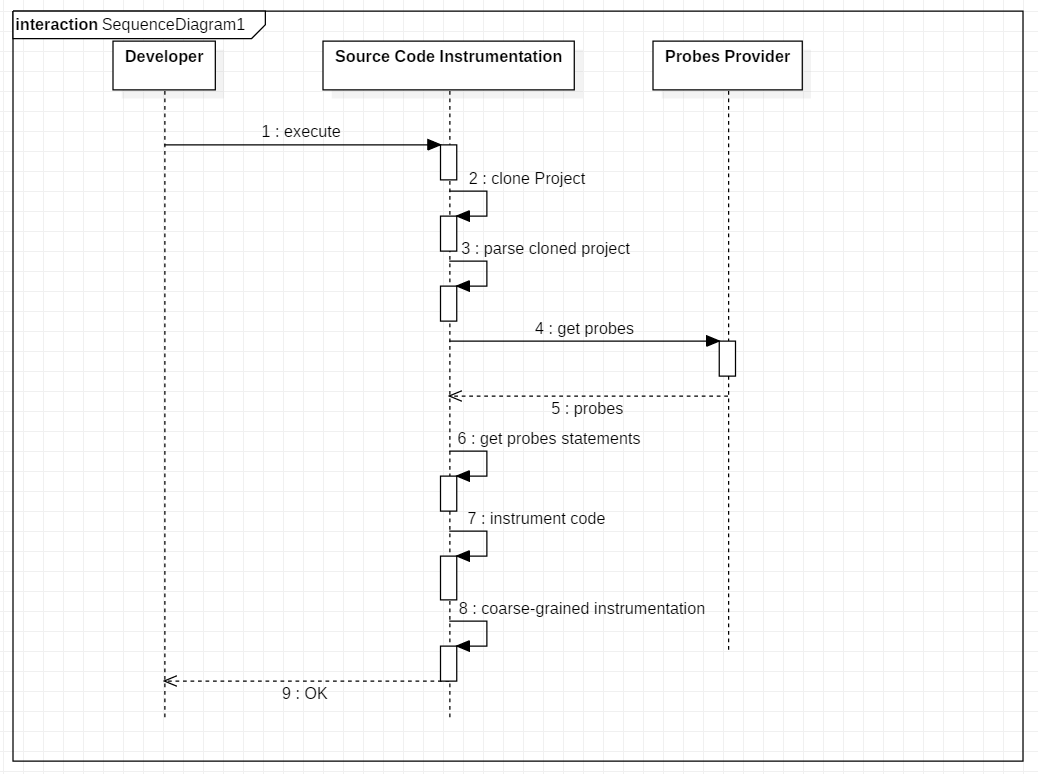
\includegraphics[width=0.9\textwidth]{figures/instrumentation_process}
\caption{Sequence Diagram that illustrates the activities of the Instrumentation Process}
\label{fig:instrumentation_process}
\end{figure}

\subsection{Service Parameters Extraction}
\label{sec:Service Parameters Extraction}
Manar and Koziolek showed in their approach \cite{mazkatli2018continuous} that Performance Model parameters can strongly depend on the parameters of the services. Therefore, we decided to enrich our monitoring information by extracting the service parameters and their values. \\

Figure \ref{fig:service_parameters} shows our approach for extracting the service parameters. We limited our approach to five parameter types, namely the type Map, Collection, Array, Primitive and Data Types. Data Types are the types that are defined by the user and are given as parameters to a service. For example, a DataType can be Java Bean Class named FileType, which contains the attributes file name of type string and file content of type Array of byte.\\

For service parameters extraction, we return for each parameter type only the property that has impact on the performance model. For collections and maps we extract their size. The same thing for arrays, we return their length. As for primitive types, we return the value of the parameter. Furthermore, Data types are handled via Reflection. In Data types we use reflection to search for attributes of the types Map, Collection, Array or Primitive in order to extract their defined properties. \\


\begin{figure}[h]
\centering
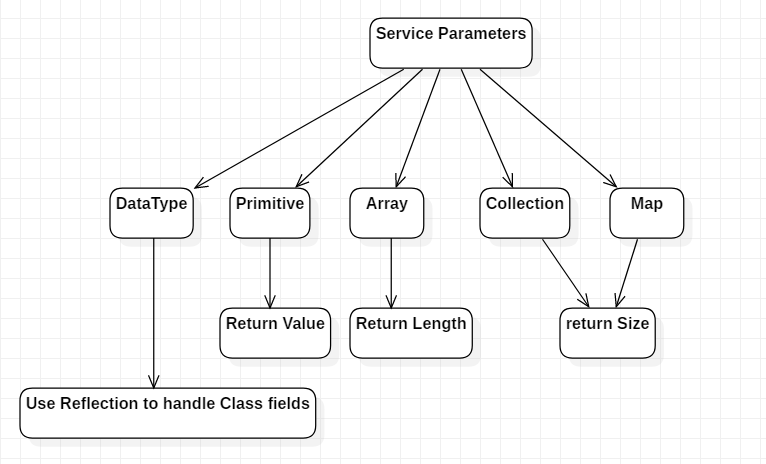
\includegraphics[width=0.9\textwidth]{figures/service_parameters}
\caption{Service parameters types and how they are extracted}
\label{fig:service_parameters}
\end{figure}


\section{Limitation}
\label{sec:Limitation}
In this section, we will present the limitation of our process for generation the monitoring probes.\\ 

\textbf{Limitation (1): adaptive Instrumentation is limited to Service level}\\
This limitation is due to the implementation of the SEFF Reconstruction Process (Section \ref{sec:Incremental SEFF Reconstruction}) which recreates the whole SEFF of a service if a part of its source code has changed. That means, if only one element of the SEFF of the changed service has been changed, the process creates a new SEFF with new elements and replaces the old SEFF of the service. This will guide to delete the old elements of the SEFF and loose their estimated parameters, even tough they were not touched by the last changes. This limitation is reflected also on the adaptive instrumentation, the adaptive monitoring and the parameters estimation of SEFF models.\\ 

Another level that can be achieved to prevent this limitation is the statement level. In this level, only the SEFF elements that was touched by the source code changes have to be updated. In such way, we can reduce the monitoring probes which reduces the overhead of the monitoring and parameters estimation of the performance model. This can be achieved for example by comparing the SEFF of the old service and the SEFF of the new service based on the source code statements. Using this comparison, we can deduce, which element of the old SEFF has been modified, new added or deleted.  \\

\textbf{Limitation (2): probes with small response time must be ignored}\\
This limitation is related to service calls and internal actions. Basically, probes with response time that do not influence the performance model must be ignored. For example, an internal action that corresponds solely to a variable declaration will clearly log response time that does not affect the performance model.\\
 
We identify basically two approaches to find out if a probe with a given response time can be accepted or ignored. The First approach consists of analyzing the statements of the source code in order to decide if the probe can affect the performance model. This approach is efficient in terms of reducing the computation resources for the instrumentation, the monitoring and the parameters estimation.  However, we do not know if it's possible to apply it for all cases.\\

The second approach, which we've implemented in our approach is the filtering of the monitoring records under a defined response time value. However, this approach is applied after monitoring phase and is less efficient then the first approach because we apply the computation resources in the monitoring of probes that are not relevant. \\

If the first approach can not cover all cases, it can be used in combination with the second approach in order to improve the efficiency of the monitoring. In the first step, the first approach can be used to remove probes that has a defined number and types of statements. In the second step, the second approach will remove the records with a defined response tine value, which could not be judged by the first approach.\\

\section{Extending the Incremental SEFF Reconstruction Process}
\label{sec:extend the incremental SEFF reconstruction process}
In this section, we will introduce our contribution in the Incremental SEFF Reconstruction Process (Section \ref{sec:Incremental SEFF Reconstruction}). The objective of our contribution is to increase the level of incrementation of the SEFF reconstruction process. Moreover, our contribution aims to reduce the high overhead caused by the monitoring of large systems.\\

Our motivation for introducing this contribution was due to the shortcoming of the Incremental SEFF Reconstruction Process that we highlighted in limitation (2) (Section \ref{sec:Limitation}). Furthermore, the incremental SEFF generation of the services is limited to service level. That means, if the source code that corresponds to one element of the SEFF elements of the service has changed, the process will create a new SEFF for the service and the remove its old SEFF. This includes removing the old elements of the SEFF even though they did not change. As consequence, we will need to repeat the monitoring for all elements of the SEFF. In respect to this, the overhead of the monitoring will increase.

\subsection{Objective}
\label{sec:objective}
In our contribution to the Incremental SEFF Reconstruction Process, we will propose an approach that resolve the limitation presented above. We will precisely extend this process by updating only the SEFF elements that have been affected by the service changes. This will prevent the recreation of the whole SEFF of the service and spare untouched SEFF elements. As results, we can minimize the overhead of the monitoring. 

\subsection{Method}
\label{sec:Method}
In order to achieve the objective presented above, we will base our approach on comparing the old and the new SEFF of the service. The old SEFF of the service can be obtained from Correspondence Model. The new SEFF of the service corresponds to the new source code of the service. The new SEFF of the service can be returned by executing the SoMoX on the new source code of the service. \\

When the source code of the service changes, we return its old SEFF and we run the SoMoX on it in order to receive the SEFF of the new source code of the service. The comparison of the old SEFF and the new SEFF of the service will provide a difference that can by analyzed in order to updated the old SEFF of the service.  

\subsection{Scientific Challenges}
\label{sec:Scientific Challenges}
In this section, we introduce the challenges that we need to solve in order to achieve the objective (Section \ref{sec:objective}) of our contribution. 

\begin{itemize}
\item How can we compare the old and the new SEFF?
\item How can we calculate the difference between the old and the new SEFF?
\item How can we update the old SEFF based on the difference between the old and the new SEFF?
\end{itemize}


\subsection{SEFF Comparison}
\label{sec:SEFF Comparison}
As mentioned above, our approach is based on the comparison of the old and the new SEFF of the service. In order to compare the SEFF elements we proposed to use their corresponding JaMoPP (section) statements in the source code. Moreover, each SEFF element is represented by a set of statements in the source code, which means, in order to compare two SEFF elements we can simply compare their statements.\\

\textbf{SPLevo: Diffing JaMoPP Cartridge}\\
In order to compare the JaMoPP statements, we used the software development tool SPLevo \cite{klatt2016consolidation}. SPLevo provides the Diffing JaMoPP functionality, which can compare between JaMoPP models. We used this functionality to compare between JaMoPP statements, which we need, in order to compare SEFFs.

\subsection{Approach}
\label{sec:approach}
Figure \ref{fig:seff_reconst_extension_level2} shows our contribution to the Incremental SEFF Reconstruction Process. The original process is described in (section in foundation). In the following we will describe the activities that we added to the process in order to achieve our objectives (Section \ref{sec:objective}). Furthermore, the activities in the blue color represent our contribution.

\textbf{Step (1): Remove all abstract actions of the old method from the correspondence model}\\
This activity is responsible for clearing the correspondence model from the old method and its correspondences. This is required because the old method will be replaced by the new method and we will need create new correspondences for the new method.\\

\textbf{Step (2): Return the Old Resource Demanding Behaviour}\\
In this step, we use the old method reference to return its SEFF from the correspondence model.\\

\textbf{Step (3): Run SoMoX to find the New Resource Demanding Behavior}\\
In this step, we run the SoMoX on the new method in order to return its SEFF. \\

\textbf{Step (4): Find the Matching of the New and the Old Resource Demanding Behavior}\\
In this step, we compute the matching between the old SEFF and the new SEFF. The matching possibilities are represented by the UML class diagram in Figure \ref{fig:seffmachting}.  The output of this step is a list of the matching between the old SEFF elements and the new SEFF elements. The enumeration \textit{MatchingType} describes the matching types, which define if two SEFF elements are totally equal or not. Two SEFF elements are total equal if their statements match completely. \\

A matching of type modified means that the source code of the old SEFF element has changed but it has a matching in the new SEFF. This type of matching will inform us, if an SEFF element has been modified.\\

\begin{figure}[h]
\centering
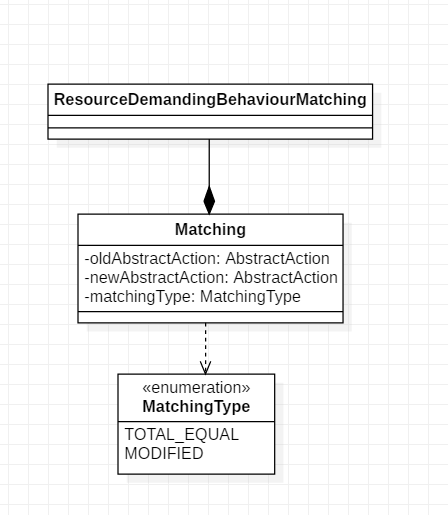
\includegraphics[width=0.9\textwidth]{figures/seffmachting}
\caption{UML class diagram that models the matching between the old and the new SEFF}
\label{fig:seffmachting}
\end{figure}


\textbf{Step (5): Find the Difference between the New and the Old Resource Demanding Behavior}\\

\begin{figure}[h]
\centering
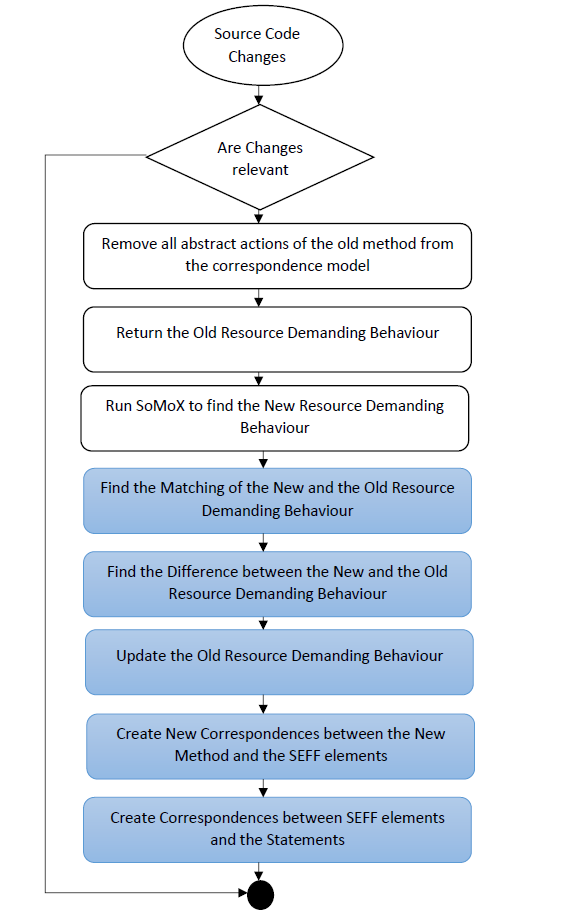
\includegraphics[width=0.9\textwidth]{figures/seff_reconst_extension_level2}
\caption{The activities in blue color shows our contribution to the Incremental SEFF Reconstruction Process \ref{sec:Incremental SEFF Reconstruction}}
\label{fig:seff_reconst_extension_level2}
\end{figure}

 
 
 